\subsection{Processing Pipeline}

Having defined the system hardware and sensor configurations, the next step is to establish the processing methodology that transforms raw sensor outputs into reliable odometry estimates.  
The proposed pipeline follows a modular structure, where each stage addresses a specific task: aligning radar frames through rigid-body transformations, merging dual-sensor data, filtering unreliable detections, clustering meaningful structures, and finally estimating ego-motion using Iterative Closest Point (ICP).  

The overall data flow is illustrated in Fig.~\ref{fig:dual_radar_pipeline}, which summarizes how radar and IMU measurements are progressively refined before contributing to odometry estimation.  
This organization enables stepwise validation, as each module can be evaluated independently before integration into the complete system.  

The following subsections present the mathematical formulations and algorithmic logic of each module in detail, supported by block diagrams to illustrate the transformations applied at each stage.  
By combining radar Doppler measurements with orientation inputs from the IMU, the pipeline is designed to deliver robust odometry even in environments where conventional vision- or LiDAR-based methods fail.

\vspace{0.5em}
\subsubsection{Rigid-Body Transformation}  
\hfill 
\\
Each radar sensor in the dual-radar configuration is physically mounted with a specific orientation and tilt relative to the vehicle's forward direction. 
To ensure a common frame of reference for all points, it is necessary to compensate for:

\begin{itemize}
    \item \textbf{Yaw rotation}: due to angled placement ($\pm30^\circ$) of the radar modules.
    \item \textbf{Pitch tilt}: due to upward mounting tilt ($15^\circ$), which must be compensated to recover horizontal geometry.
    \item \textbf{Sensor offset}: due to the physical separation of the radar sensors in the horizontal axis (X-axis).
\end{itemize}

\vspace{0.5em}
\paragraph{Yaw Correction (Z-axis Rotation)}
The radar sensors are rotated relative to the vehicle frame:

\begin{itemize}
    \item Radar A (Left): Mounted at $+30^\circ$ yaw $\Rightarrow$ compensated with $-30^\circ$ rotation.
    \item Radar B (Right): Mounted at $-30^\circ$ yaw $\Rightarrow$ compensated with $+30^\circ$ rotation.
\end{itemize}

The 2D rotation in the XY-plane is defined as:
\[
\begin{bmatrix}
x' \\
y' \\
z'
\end{bmatrix}
=
\begin{bmatrix}
\cos(\theta) & -\sin(\theta) & 0 \\
\sin(\theta) & \cos(\theta) & 0 \\
0 & 0 & 1
\end{bmatrix}
\begin{bmatrix}
x \\
y \\
z
\end{bmatrix}
\]

where $\theta = \pm30^\circ$ depending on the sensor.

\begin{figure}[!htbp]
    \centering
    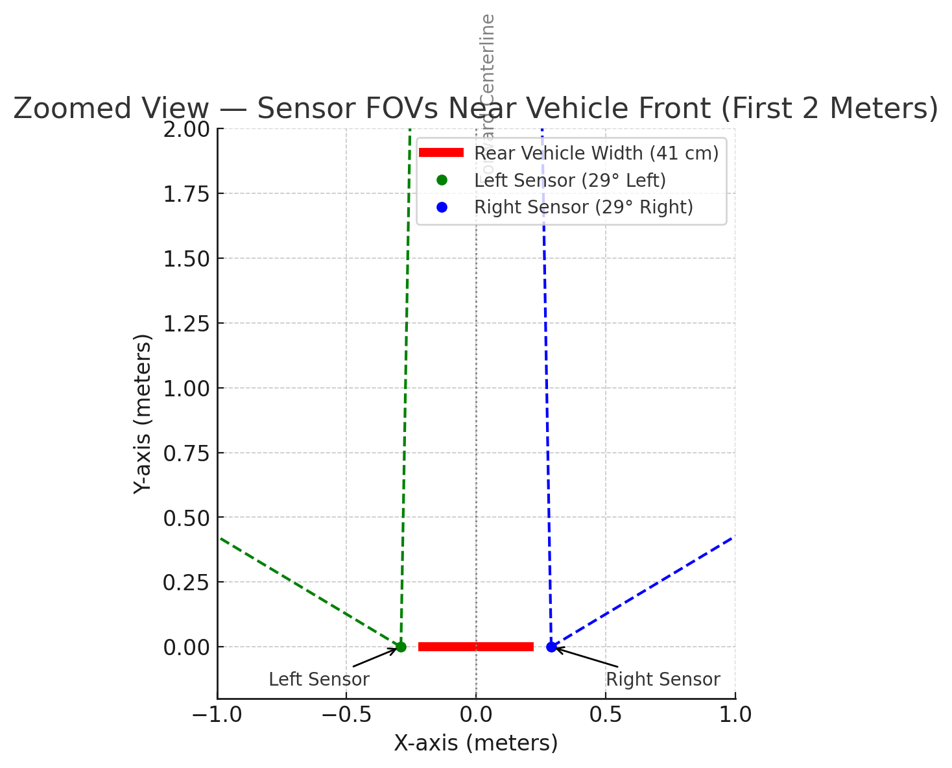
\includegraphics[width=0.8\linewidth]{images/SensorsRotation.png}
    \caption{Simulation of yaw rotation of sensors around the Z-axis ($\pm30^\circ$).}
    \label{fig:z_axis_rotation}
\end{figure}

\begin{figure}[!htbp]
    \centering
    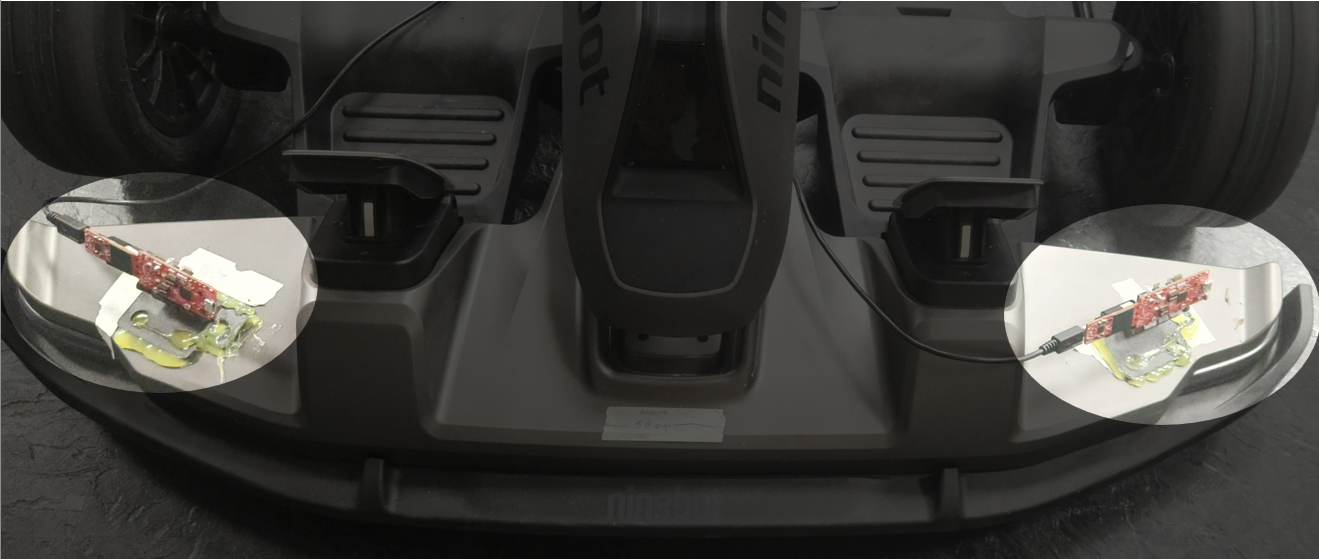
\includegraphics[width=0.8\linewidth]{images/vehicleRadarYawRotationHighlited.png}
    \caption{Real-world implementation of yaw rotation in the vehicle.}
    \label{fig:vehicleRadarYawRotation}
\end{figure}


The yaw angles of $\pm30^\circ$ were selected through a combination of physical measurement and simulation of the sensor field of view (FOV).  
Using the vehicle chassis centerline as a reference, the mounted sensors were visually measured to exhibit a yaw of approximately $28$--$32^\circ$ outward (see Fig.~\ref{fig:vehicleRadarYawRotation}), which confirmed the intended target of $30^\circ$ opening from the vehicle center.  
This estimate was further cross-checked in simulation by plotting the radar FOV using the TI Demo Visualizer, which allows configuration of the theoretical horizontal FOV from its default $90^\circ$ down to $60^\circ$ or $30^\circ$ respectfully.  
\begin{comment}
    Add picture of this validation
\end{comment}
The $60^\circ$ configuration was adopted as it provides improved angular resolution while discarding irrelevant detections outside the useful sector.  
Within this setting, the $\pm30^\circ$ mounting maximizes the combined coverage of the dual-radar system, while creating a small blind zone of approximately $4$~m directly in front of the vehicle.  
This trade-off was deliberately accepted to ensure the widest effective overlap of both radars for odometry tasks.

\vspace{0.5em}
\paragraph{Pitch Compensation (X-axis Rotation)}
Since the radar sensors are tilted upward by $15^\circ$, a corrective rotation around the X-axis is applied to bring the points back to a horizontal perspective: 

\[
\begin{bmatrix}
x' \\ y' \\ z'
\end{bmatrix}
=
\begin{bmatrix}
1 & 0 & 0 \\
0 & \cos(\phi) & -\sin(\phi) \\
0 & \sin(\phi) & \cos(\phi)
\end{bmatrix}
\begin{bmatrix}
x \\ y \\ z
\end{bmatrix}
\]

where $\phi = -15^\circ$ (negative to reverse the upward tilt).

\begin{figure}[!htbp]
    \centering
    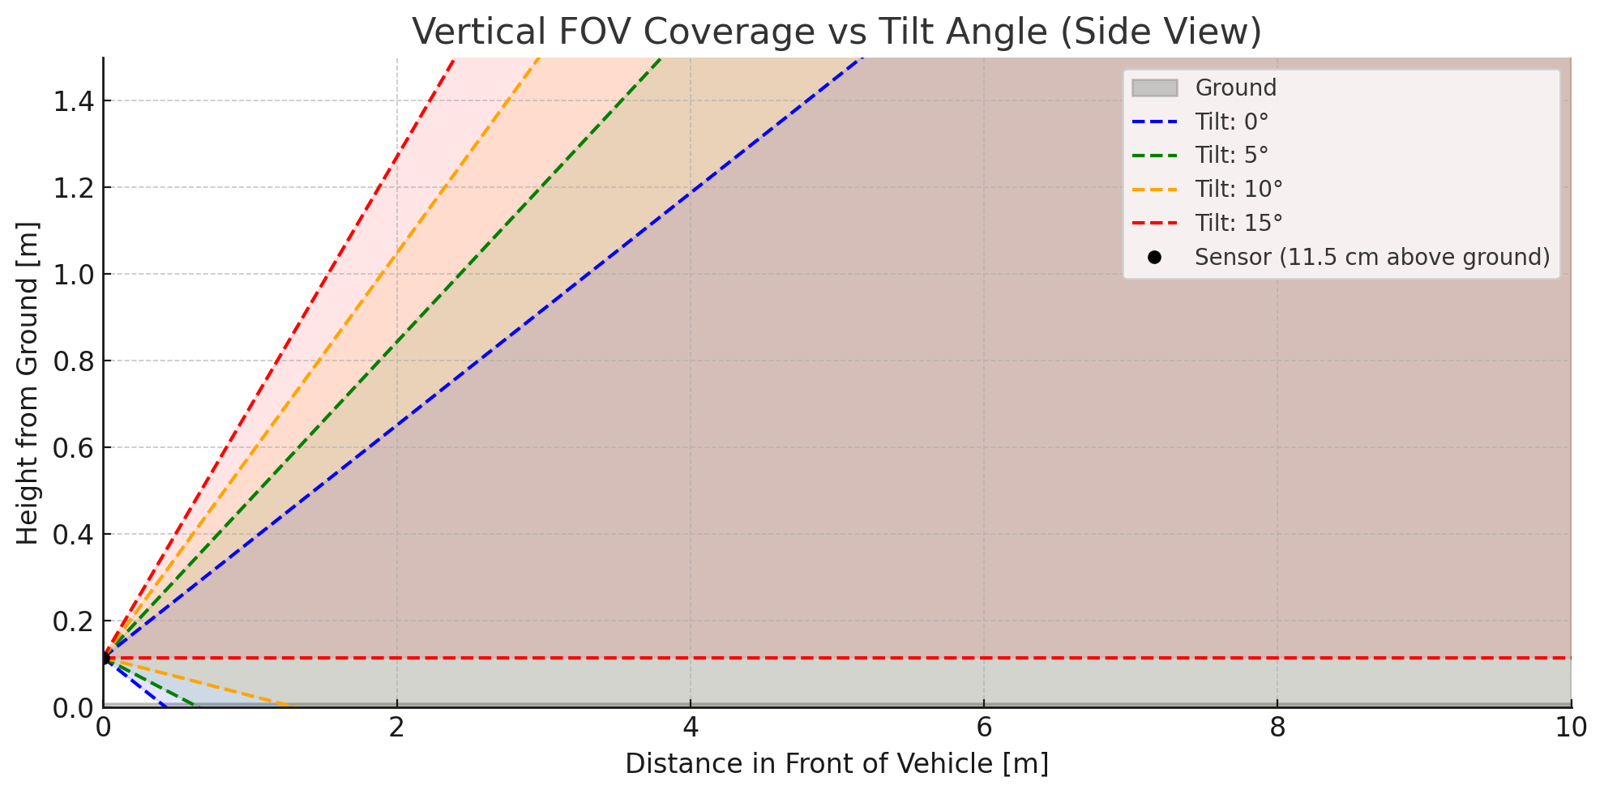
\includegraphics[width=0.8\linewidth]{images/TiltSensor.png}
    \caption{Pitch compensation for $15^\circ$ upward tilt.}
    \label{fig:x_axis_rotation}
\end{figure}

The upward tilt of $15^\circ$ was introduced to minimize clutter from the ground plane.  
With the sensor's vertical FOV of approximately $30^\circ$, this configuration reduced spurious reflections while maintaining sufficient detection of obstacles at the intended height range.  
Both the yaw and pitch choices were tested through simulation and validated in real-world mounting experiments (Figures~\ref{fig:z_axis_rotation}, \ref{fig:vehicleRadarYawRotation}, \ref{fig:x_axis_rotation}, \ref{fig:vehicleYawTilt}).

\begin{figure}[!htbp]
    \centering
    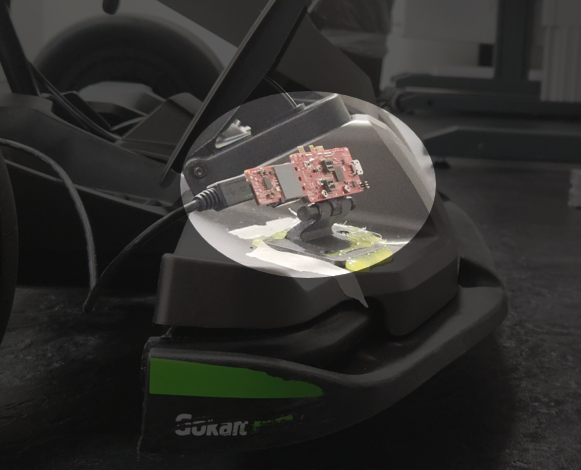
\includegraphics[width=0.8\linewidth]{images/vehicleRadarTiltRotation.png}
    \caption{Real-world implementation of radar tilt ($15^\circ$ upward).}
    \label{fig:vehicleYawTilt}
\end{figure}

\paragraph{X-Axis Offset Compensation}
After rotation, each sensor's point cloud was translated along the X-axis to align with the vehicle's center:
\begin{itemize}
    \item Radar A: $x \leftarrow x - 0.32$ meters
    \item Radar B: $x \leftarrow x - 0.28$ meters
\end{itemize}

This translation ensured both sensors were aligned in a common vehicle-centric frame.

\begin{figure}[!htbp]
    \centering
    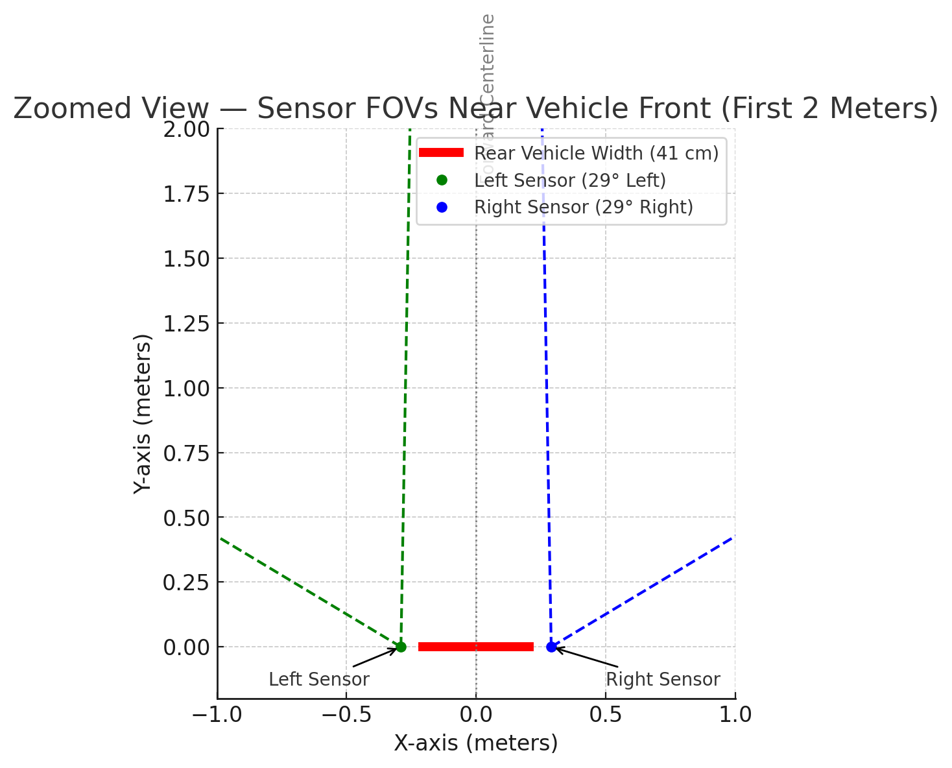
\includegraphics[width=0.8\linewidth]{images/RotationSensor.png}
    \caption{Final extrinsic configuration combining yaw, pitch, and translation.}
    \label{fig:extrinsics}
\end{figure}

A yaw rotation \( R_{\text{yaw}} \) was first implemented, followed by a pitch correction \( R_{\text{pitch}} \), and finally a translation vector \( \vec{t} \) was applied to account for the physical position of the sensors with respect to the vehicle's coordinate origin.

The full transformation can be expressed as:

\begin{equation}
T_{\text{veh}} = R_{\text{yaw}} \cdot R_{\text{pitch}} \cdot \vec{p}_{\text{radar}} + \vec{T}
\label{eq:radar_to_vehicle_transform}
\end{equation}

Where:
\begin{itemize}
    \item \( \vec{p}_{\text{radar}} \) is a radar point in sensor coordinates.
    \item \( R_{\text{yaw}} \) is a 2D rotation around the vertical axis ($\pm30^\circ$).
    \item \( R_{\text{pitch}} \) corrects for the upward sensor tilt ($-15^\circ$).
    \item \( \vec{T} \) is the translation vector.
\end{itemize}

\paragraph{Summary of Extrinsics}
\begin{itemize}
    \item \textbf{Left radar:} yaw $+30^\circ$, pitch $-15^\circ$, translation $(-0.32, 0, 0)$.
    \item \textbf{Right radar:} yaw $-30^\circ$, pitch $-15^\circ$, translation $(-0.28, 0, 0)$.
\end{itemize}

This extrinsic calibration ensures that dual-radar data is expressed in a coherent vehicle-centric frame, which is critical for downstream modules such as clustering, odometry, and obstacle tracking.

\vspace{0.5em}
\subsubsection{Radar Merge}  
\hfill 
\\
\indent Once each radar's detections were transformed into the common vehicle frame, the two datasets were merged into a single unified point cloud per frame.  
This step ensured that detections from both radars contributed consistently to the pipeline.  

This fusion improves both density and coverage, particularly in regions where the individual radar fields of view overlap.  
It also reduces ambiguity during clustering, since targets detected by both sensors reinforce one another once aligned.  

The effect of merging is visualized in Fig.~\ref{fig:radar_merge}, where the independent point clouds (top) are combined into a single dataset (bottom).  

\begin{figure}[!htbp]
    \centering
    \begin{subfigure}[t]{0.8\linewidth}
        \centering
        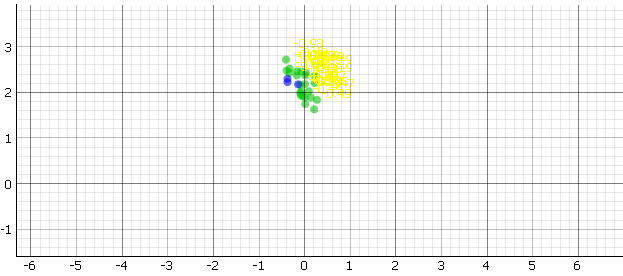
\includegraphics[width=\linewidth]{images/AFTERdualSensorCalib_2mts.png}
        \caption{Independent point clouds before merging.}
    \end{subfigure}
    \vfill
    \begin{subfigure}[t]{0.8\linewidth}
        \centering
        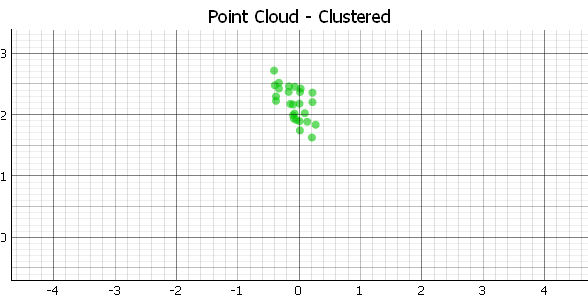
\includegraphics[width=\linewidth]{images/AFTERdualSensorCalibCluster_2mts.png}
        \caption{Unified point cloud after merging.}
    \end{subfigure}
    \caption{Radar merge process: alignment of calibrated detections into a single dataset.}
    \label{fig:radar_merge}
\end{figure}

\vspace{0.5em}
\subsubsection{Frame Aggregator}  
\hfill 
\\
The frame aggregator addresses the inherent sparsity of single radar frames by combining multiple consecutive frames into a denser and more reliable point cloud.  
While aggregation increases both useful information and noise, it ultimately improves object reconstruction, motion estimation, and detection stability.

\paragraph{Single Frame}
Processing a single frame often leads to incomplete or fragmented detections:
\begin{itemize}
    \item Objects may not be fully represented due to the low number of points.
    \item Close objects can merge or be misclassified because of insufficient separation in sparse data.
\end{itemize}

\begin{figure}[!htbp]
    \centering
    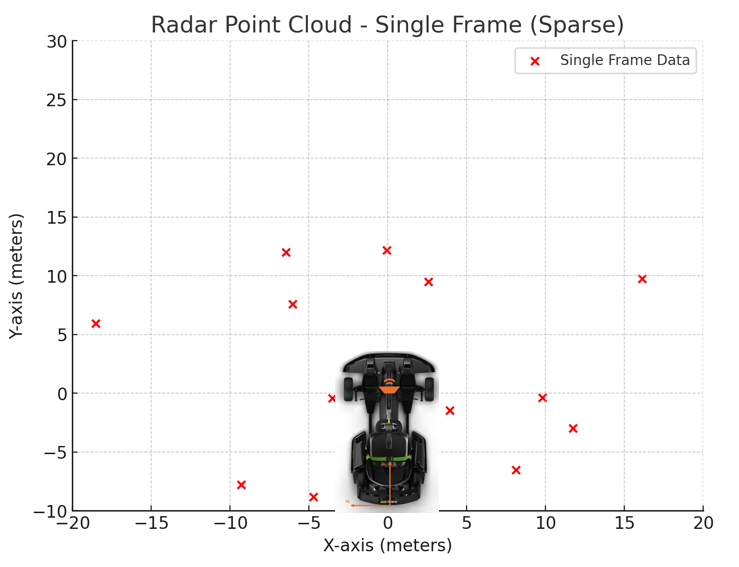
\includegraphics[width=0.5\linewidth]{images/singleframe.png}
    \caption{Single-frame visualization.}
    \label{fig:single_frame}
\end{figure}

This sparsity-induced ambiguity is not a limitation of the clustering algorithms themselves, but a direct consequence of limited raw data.

\paragraph{Multiple Frames}
To mitigate these issues, multiple frames are aggregated in a fixed-size buffer, where older frames are removed as new ones arrive.  
This method increases point cloud density, reduces variance as per the Law of Large Numbers, and stabilizes detections:
\begin{equation}
    \frac{\sigma^2}{N}
    \label{eq:variance_per_sample_size}
\end{equation}

\begin{figure}[!htbp]
    \centering
    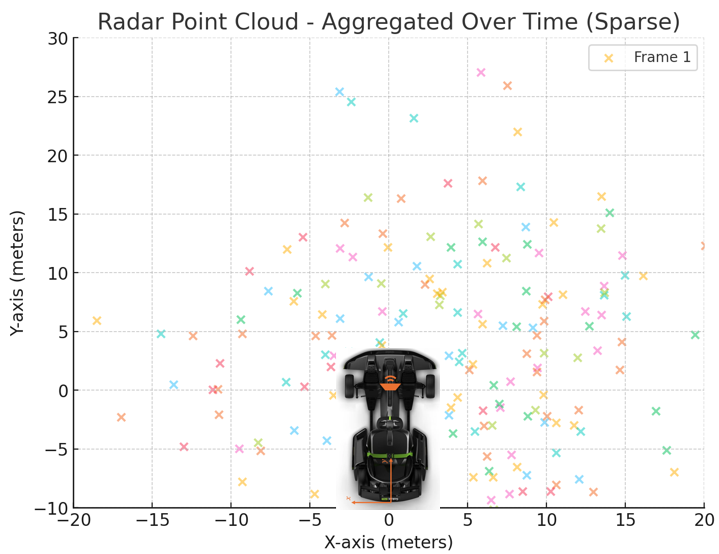
\includegraphics[width=0.5\linewidth]{images/multiframe.png}
    \caption{Multi-frame aggregation visualization.}
    \label{fig:multiframe}
\end{figure}

During experimentation, the number of aggregated frames was varied between 7 and 15.  
A value of 10 frames provided the best balance: enough temporal density to reduce noise and reveal stable structures, while minimizing the persistence of outdated points.  
This configuration was therefore adopted for all subsequent pipeline stages.

\vspace{0.5em}
\subsubsection{Filtering Stage: $y$-axis and Doppler}
\hfill 
\\
The raw radar point cloud exhibited systematic clutter in the region directly in front of the sensors, primarily due to reflections from the driver’s feet and the ground.  
These unwanted detections were consistently observed up to approximately \SI{1.5}{\meter} and persisted even when the vehicle was stationary.  
If left unfiltered, such clutter propagated through the pipeline, degrading clustering and motion estimation.  

To address this, a static filtering stage was implemented with two criteria:
\begin{enumerate}
    \item \textbf{$y$-axis filter:} Only points within the interval $1.5 \leq y \leq 15$~m are retained.  
    This introduces a \textit{dead zone} in front of the vehicle, removing ground clutter and very short-range reflections while keeping the operational range relevant for odometry.
    \item \textbf{Doppler filter:} Only points with radial velocity within $0.01 \leq v_d \leq 8.0$~m/s are accepted.  
    This rejects near-zero Doppler detections (often noise or static artifacts) and unrealistically large outliers.
\end{enumerate}

\noindent
This filtering approach significantly reduced spurious reflections (Fig.~\ref{fig:filter_example}), producing a cleaner point cloud for downstream modules.  
The trade-off is that genuine obstacles appearing within the \SI{1.5}{\meter} dead zone are excluded.  
Although this removes potentially useful information in very close range, the region is dominated by ground clutter and considered less critical for the odometry pipeline.  

\begin{figure}[!htbp]
    \centering
    \begin{subfigure}{0.45\linewidth}
        \centering
        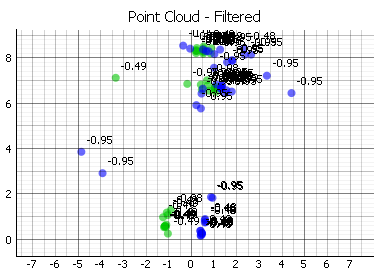
\includegraphics[width=\linewidth]{images/dualSensorClutterYAxis.png}
        \caption{Clutter representation (Radar~A = blue, Radar~B = green).}
        \label{fig:clutter_representation}
    \end{subfigure}
    \hfill
    \begin{subfigure}{0.45\linewidth}
        \centering
        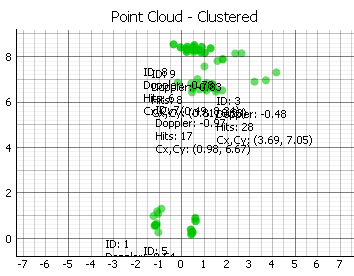
\includegraphics[width=\linewidth]{images/dualSensorClutterYAxisCluster.png}
        \caption{Clustered view of clutter detections.}
        \label{fig:clutter_clustered}
    \end{subfigure}
    \caption{Visualization of unwanted reflections (clutter) near the sensors, dominated by ground and driver-related reflections up to \SI{1.5}{\meter}.  
    Blue dots correspond to Radar~A (left), and green dots to Radar~B (right).}
    \label{fig:filter_example}
\end{figure}


\FloatBarrier


\subsubsection{RANSAC-Based Motion Filtering}

A critical step in radar-based odometry is separating static landmarks from dynamic objects, ensuring ego-motion is derived only from stable references.  
This is achieved through a RANSAC-based filtering method applied to the relationship between azimuth angle $\theta$ and Doppler velocity $v_d$.

\paragraph{Principle}
When mounted on a moving vehicle, static objects do not appear motionless: they exhibit Doppler velocities that vary smoothly with azimuth, forming a predictable distribution in the $\theta$–$v_d$ plane.  
Dynamic objects deviate from this distribution and appear as outliers.  

RANSAC (Random Sample Consensus) robustly fits a model to this distribution, identifying inliers (static reflections) and outliers (moving targets).  
At this stage no ego-speed estimation has yet been performed — RANSAC provides the static/dynamic separation required before estimating the vehicle’s own velocity.

\paragraph{Mathematical Model}
Ideally, the Doppler relation for static points follows
\[
v_d = v_e \cos(\theta),
\]
where $v_e$ is the ego velocity.  
However, this direct form is impractical because $v_e$ is not known a priori and sensor misalignments, calibration errors, and noise distort the ideal cosine curve.  

Instead, the relationship is approximated as a quadratic:
\[
v_d = a\theta^2 + b\theta + c,
\]
fitted using RANSAC.  
This choice offers two advantages:
\begin{itemize}
    \item \textbf{Robustness to real-world distortions:} the polynomial can absorb small yaw/pitch offsets and clutter that shift the ideal cosine.
    \item \textbf{Independence from $v_e$:} the fit does not require prior knowledge of ego speed, which is only derived after static inliers are identified.
\end{itemize}

Thus, the polynomial model is a practical compromise: flexible enough to capture the Doppler trend without assuming known vehicle speed.

\paragraph{Integration into the Pipeline}
The RANSAC filter is applied after static $y$-axis and Doppler thresholding.  
It outputs:
\begin{itemize}
    \item \textbf{Inliers:} static reflections, passed to clustering and later used for ICP and ego-velocity estimation,
    \item \textbf{Outliers:} dynamic objects, excluded from motion estimation.
\end{itemize}

\begin{figure}[!htbp]
    \centering
    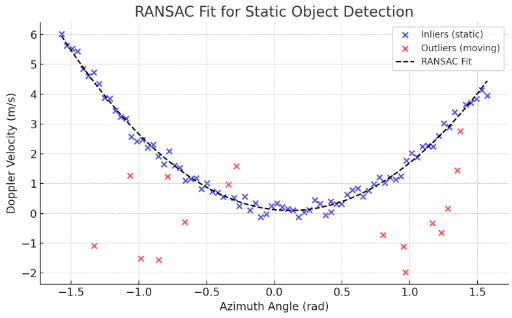
\includegraphics[width=1.0\linewidth]{images/RANSAC.png}
    \caption{RANSAC fit of Doppler vs. azimuth. Inliers = static (blue), Outliers = moving (red).\\
    \textit{Note: This figure uses simulated data to illustrate the concept.}}
    \label{fig:ransac_simulated_static_dynamic}
\end{figure}

\begin{figure}[!htbp]
    \centering
    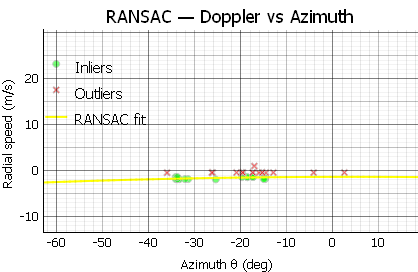
\includegraphics[width=1.0\linewidth]{images/RANSAC_movingTarget_wPtCloud.png}
    \caption{RANSAC fit of Doppler vs. azimuth. Inliers = static (green), Outliers = moving (red).\\
    \textit{Note: This figure shows real data when the vehicle is moving and a dynamic target is present.}}
    \label{fig:ransac_real_static_dynamic}
\end{figure}

\begin{figure}[!htbp]
    \centering
    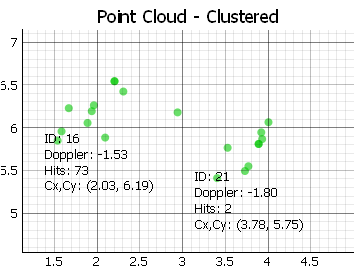
\includegraphics[width=1.0\linewidth]{images/RANSAC_movingTarget_ptCloud.png}
    \caption{Clustered point cloud corresponding to the RANSAC analysis in Fig.~\ref{fig:ransac_real_static_dynamic}. 
    Each cluster is annotated with ID, Doppler average, and centroid coordinates.}
    \label{fig:ransac_clustered_ptcloud}
\end{figure}

\begin{figure}[!htbp]
    \centering
    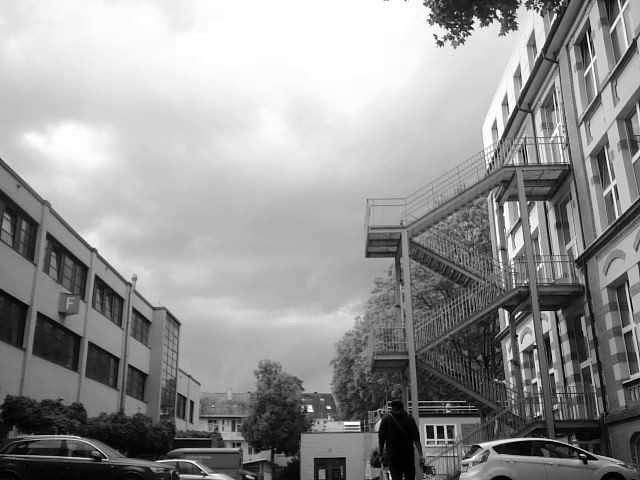
\includegraphics[width=1.0\linewidth]{images/frame_15s.png}
    \caption{Video frame at $t=15$ seconds, showing the target in the scene. 
    This frame corresponds to the radar data used in Figs.~\ref{fig:ransac_real_static_dynamic} and \ref{fig:ransac_clustered_ptcloud}.}
    \label{fig:frame_15s_target}
\end{figure}

\paragraph*{Benefits}
\begin{itemize}
    \item Robust to clutter and noise,
    \item Separates dynamic actors without prior labeling,
    \item Provides the static inlier set required for ego-speed estimation, clustering, and ICP alignment.
\end{itemize}

By anchoring odometry on static inliers, RANSAC prevents dynamic objects from corrupting trajectory estimation and ensures robustness in cluttered or mixed-traffic scenarios.
